\documentclass{ctexart}
\usepackage{graphicx}
\usepackage{subfigure}
\CTEXsetup[format+={\flushleft}]{section}

\begin{document}
\CJKfamily{li}
\title{周报}
\author{刘精昌}
\maketitle

\fangsong
\section*{本周工作}
\begin{itemize}
  \item 阅读周志华《机器学习》第十六章强化学习。
  \item 通过有论文性质的官方文档《Computing and Visualizing Dynamic Time Warping Alignments in R: The dtw Package》,学习了R语言里面的dtw包。dtw包是衡量序列距离的dtw方法的R语言实现。dtw包的内容极其丰富,其中的一些功能包括:
      \begin{enumerate}
        \item 选择dtw的迭代方式。
        \item package提供不同的弯曲曲线边际限制的选项。
        \item 如果时间序列中的点是多维的,dtw能够提供不同的距离测度选项。
        \item package能够提供丰富的输出结果,不但能够输出dtw距离,还能输出对齐轨迹上的点等诸多信息。
        \item package能做出图1、图2所示的精美图形。
      \end{enumerate}
  \item 利用MATLAB,用人造数据,从1-NN分类准确度等角度,比较dtw、欧式距离。实验需要进一步改进。一项实验数据,是在一列相等的数上添加随机扰动产生的。分别利用dtw和欧式距离进行聚类工作,两者结果都特别好,进行1-NN 分类实验时,两者的结果都不好。对于这两种极端的实验结果,可能是数据选择不佳以及dtw的参数选择不佳造成的。实验需要从这些方面改进,而且需要进一步在其他方面实验。
  \item 阅读《Three Myths about Dynamic Time Warping Data Mining》SDM2005。论文很短,通过实验给出以下3个结论:
      \begin{enumerate}
        \item 针对dtw能处理不同长度的序列这个优点,论文认为,通过插值使得序列等长,再计算dtw距离,并不比直接计算dtw距离差。
        \item 针对warping window大小这个问题,论文认为,比较小的warping window(4\%左右)较佳.
        \item 通过更紧的下界来减小计算几乎徒劳。
      \end{enumerate}
\end{itemize}

\section*{下周计划}
\begin{itemize}
  \item 尝试开始写毕业设计论文。
  \item 改进实验并且继续做实验。
  \item 灵活地阅读书籍以及相关文献。
\end{itemize}

\begin{figure}
    \centering
    \begin{minipage}[t]{0.4\linewidth}
    \centering
    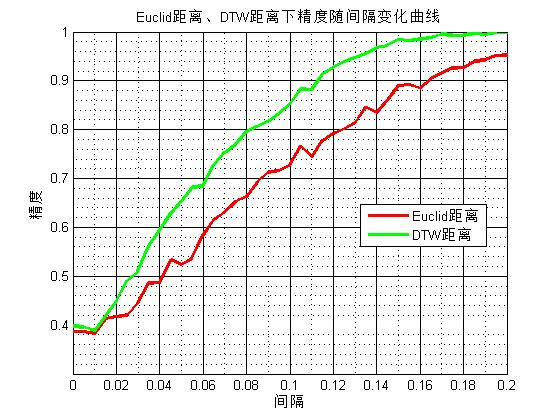
\includegraphics[width=2.2in]{1.jpg}
    \caption{Two-way plot}
    \label{fig:side:a}
    \end{minipage}%
    \begin{minipage}[t]{0.4\linewidth}
    \centering
    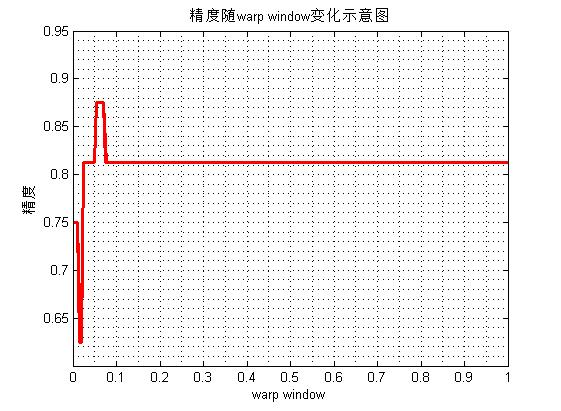
\includegraphics[width=2.2in]{2.jpg}
    \caption{Three-way plot}
    \label{fig:side:b}
    \end{minipage}
\end{figure}
\end{document} 